\documentclass[10pt,a4paper]{article}
\usepackage[utf8]{inputenc}

% \usepackage{ngerman}  % german documents
\usepackage{graphicx}  % import graphics einbinden
\usepackage{listings}  % support source code listing
\usepackage{amsmath}  % math stuff
\usepackage{amssymb} % 
\usepackage{a4wide} % wide pages
\usepackage{fancyhdr} % nice headers
\lstset{basicstyle=\footnotesize,language=Python,numbers=left, numberstyle=\tiny, stepnumber=5,firstnumber=0, numbersep=5pt} % set up listings
\pagestyle{fancy}             % header
\setlength{\parindent}{0pt}   % no indentation

\usepackage[pdfpagemode=None, colorlinks=true,  % url coloring
           linkcolor=blue, urlcolor=blue, citecolor=blue, plainpages=false, 
           pdfpagelabels,unicode]{hyperref}
           
% change enums style: first level (a), (b), (c)           
\renewcommand{\labelenumi}{(\alph{enumi})}
\renewcommand{\labelenumii}{(\arabic{enumii})}

%lecture name
\newcommand{\lecture}{
	Bioinformatics III
}           

%assignment iteration
\newcommand{\assignment}{
	Second Assignment
}

%set up names, matricle number, and email
\newcommand{\authors}{
  \begin{tabular}{rl}
    \href{mailto:s9alfloh@stud.uni-saarland.de}{Alexander Flohr} & (2549738)\\
    \href{mailto:s9ankupi@stud.uni-saarland.de}{Andrea Kupitz} & (2550260)
  \end{tabular}
}

% use to start a new exercise
\newcommand{\exercise}[1]
{
  \stepcounter{subsection}
  \subsection*{Exercise \thesubsection: #1}

}

\begin{document}
\title{\Large \lecture \\ \textbf{\normalsize \assignment}}
\author{\authors}

\setlength \headheight{25pt}
\fancyhead[R]{\begin{tabular}{r}\lecture \\ \assignment \end{tabular}}
\fancyhead[L]{\authors}


\setcounter{section}{2} % modify for later sheets, i.e. 2, 3, ...
%\section{Introduction to Python and some Network Properties} % optional, note that section invocation sets the section counter + 1, so adapt the setcounter command
\maketitle

\exercise{The scale-free network}
\begin{enumerate}
\item Listing \ref{ex1-1} shows source code.
\lstinputlisting[label=ex1-1,caption={Example Listing of source code}] {ScaleFreeNetwork.py}

\item Listing \ref{ex1-2} shows source code.
\lstinputlisting[label=ex1-2,caption={Example Listing of source code}] {Assign2Task1.py}
Both degree distributions, the one for 1000 and 10000 nodes, follow the same distribution. Only the network with more nodes has some nodes with a higher degree than the other network which seems to result from the higher number of nodes. Figure \ref{fig-1} shows the plot.
\begin{figure}
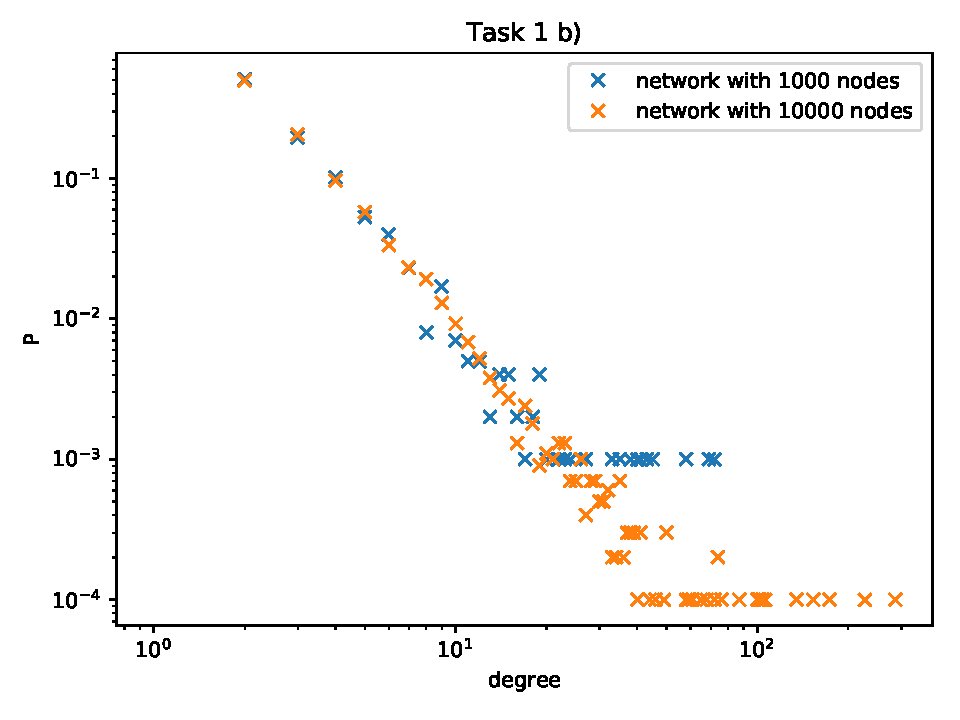
\includegraphics[scale=1]{Figure_1.pdf}
\caption{Comparison of two scale-free networks}
\label{fig-1}
\end{figure}

\item Listing \ref{ex1-3} shows source code.
\lstinputlisting[label=ex1-3,caption={Example Listing of source code}] {Tools.py}
Comparing the empirical and the theoretical distributions, one may see the first third of the graph fit well, whereas the rest of the empirical distribution is very differently distributed. We determined a gamma value of 1.8. The quality of our fit isn't very high. Maybe it could be improved by computing a average distance between each value. Figure \ref{fig-3} shows the plot.
\begin{figure}
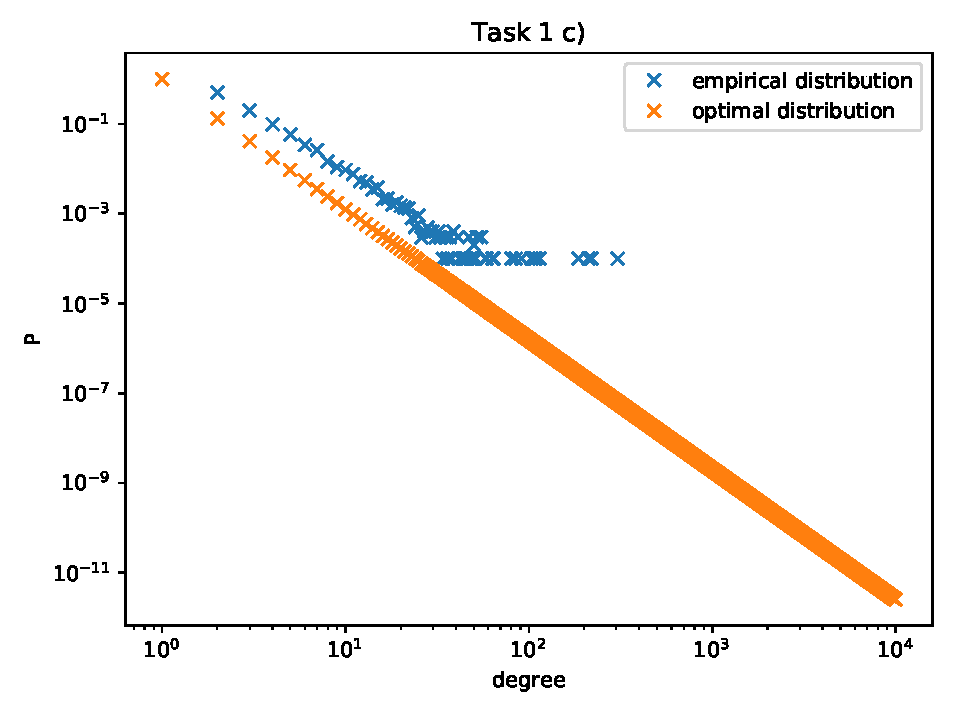
\includegraphics[scale=1]{Figure_3.pdf}
\caption{Comparison of empirical to theoretical network}
\label{fig-3}
\end{figure}
\end{enumerate}

\exercise{Real-world network}
\begin{enumerate}
\item File sharing services like Google Drive form clustered networks, which are clustered by the users which have access to a file. Every time a user adds a new file, a directed link connects a new file to an user.
\item Social networks like Facebook, Twitter and so on may be represented as undirected scale-free networks because people with many friends are more likely to get new friends because they know many people. Moreover a connection between two users is not directed because both users have to accept a friend request.\\
A social network can also be represented as a clustered network, whereby the clustered are made of different groups of friends.
\item Broadcasting networks may form hierarchical or clustered networks. In the case of a hierarchical network, we assume that one broadcaster sends data to multiple other services which publish the data. The network could be clustered by the receiver, which receive data from the same broadcaster. A directed node connects each broadcaster to its receiver.
\end{enumerate}

\exercise{Real interaction networks}
\begin{enumerate}
\item 
\item 
\item 
\item 
\end{enumerate}
\end{document}